%--------------------------------     NÃO ALTERAR    ----------------------------------------%
\begin{center}

\begin{table}[!h]
\centering
\resizebox{\textwidth}{!}{
\begin{tabular}{lr}
\multirow{6}{*}{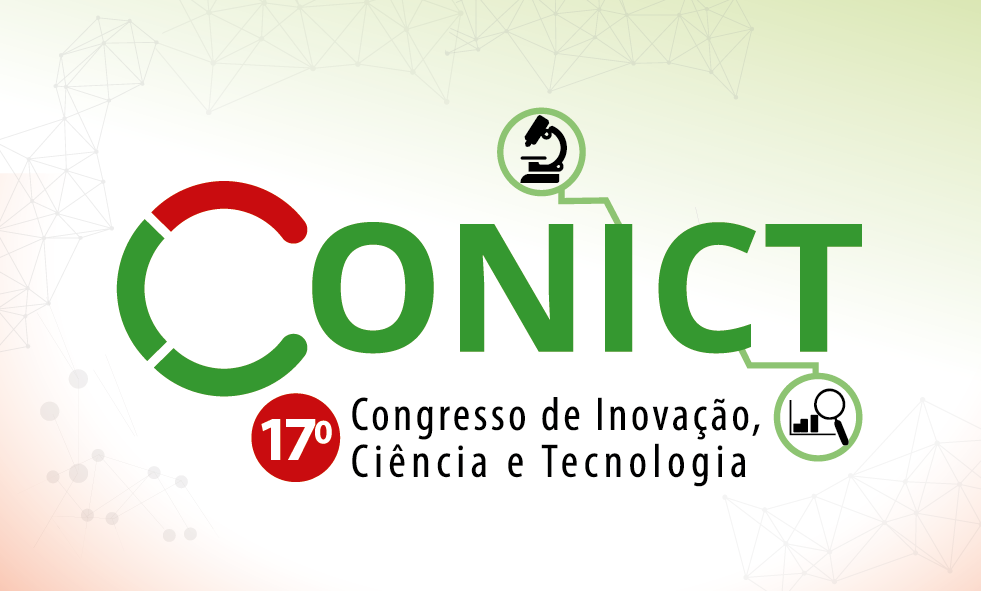
\includegraphics[width=80px]{destaque_17_conict.png}}                                                                     & \multirow{5}{*}{
\includegraphics[width=190px]{logo_reitoria.png}} \\
                        &                                                        %                    &            
                        \\
                        &                                                         %                                    &                         
                        \\
                        & \multicolumn{1}{l}{\textbf{}}                          %                                     &                        
                        \\
                        & \multicolumn{1}{l}{\textbf{}}                          %                                     &                        
                        \\
                        %& 
                        \multicolumn{2}{c}{\large{\textbf{17º Congresso de Inovação, Ciência e Tecnologia do IFSP - 2026}}} \\
                        \multicolumn{2}{c}{\textbf{Campus Guarulhos}} \\
                        %& \multicolumn{1}{l}{}   
\end{tabular}
}

\end{table}

%-------------------------------------------------------------------------------------------------%

\textbf{DETECÇÃO DE CONFORMIDADE DE SEGURANÇA EM AMBIENTES UTILIZANDO A ARQUITETURA YOLO E ACELERAÇÃO OPENVINO}\vspace{0.5cm}

KELVIN A. APARECIDO$^1$, RICARDO SOVAT$^2$

\end{center}

\begingroup
    \fontsize{9pt}{11pt}\selectfont
  
  $^1$Graduando em Tecnologia de Análise e Desenvolvimento de Sistemas, IFSP, Câmpus Campinas, \url{albuquerque.aparecido@aluno.ifsp.edu.br}.
  
  $^2$Prof. Dr. Ricardo Sovat (Orientador), IFSP, Câmpus Campinas.

  \vspace{0.2cm}
  \noindent Área de conhecimento (Tabela CNPq): 1.03.03.04-9 Sistemas de Informação. 
\endgroup
